
\subsection{背景}
%パラ言語情報について
対話場面における情報伝達は複雑である。これは音声には様々な情報が含まれており、会話時には話し手と聴き手の間に高度なやりとりがなされているためである。
音声に含まれる情報は、言語情報、パラ言語情報、非言語情報の三つに分類することができる。以下に藤崎による3分類を引用する。言語情報とは、書き言葉によって明示的に表現される情報や文脈から一意かつ容易に推測することが可能である情報のことを指す。パラ言語情報とは、書き言葉に転写すると推測不可能となる情報で、言語情報を補助ないし変容するために話者が意図的に生成する情報のことを指す。特に発話に込められた話者の意図、態度や発話のスタイルなどが該当する。非言語情報とは、話者の年齢、性別、個人性、身体ないし感情の状態などの要因に関わる情報のことを指す。これらの要因は、発話の言語的・パラ言語的内容とは直接に関係せず、話者が意図的に制御することも一般には不可能である\cite{fujisaki}。
これら三つの情報を伝達するときに、話し手と聴き手の音声伝達の模式図を図\ref{maekawa_onsei:fig}に示す。
図\ref{maekawa_onsei:fig}では、聴き手においてパラ言語情報と非言語情報が必ずしも正確に知覚されるとは限らないため、破線の矢印で示されている。パラ言語情報の影響は発話全体にわたって顕在化することもあるが、むしろ多くは発話の冒頭や末尾において局所的に顕在化している\cite{maekawa_kitagawa}。パラ言語情報を分析するためには、発話全体を対象とすることが有効であることが示されている。

このように、音声が伝える情報について研究が行われてきたが、パラ言語情報や非言語情報がどのような仕組みで生成され、伝達されているのかについて全てを明らかにすることはできていない。

\begin{figure}[hbtp]
 \centering
   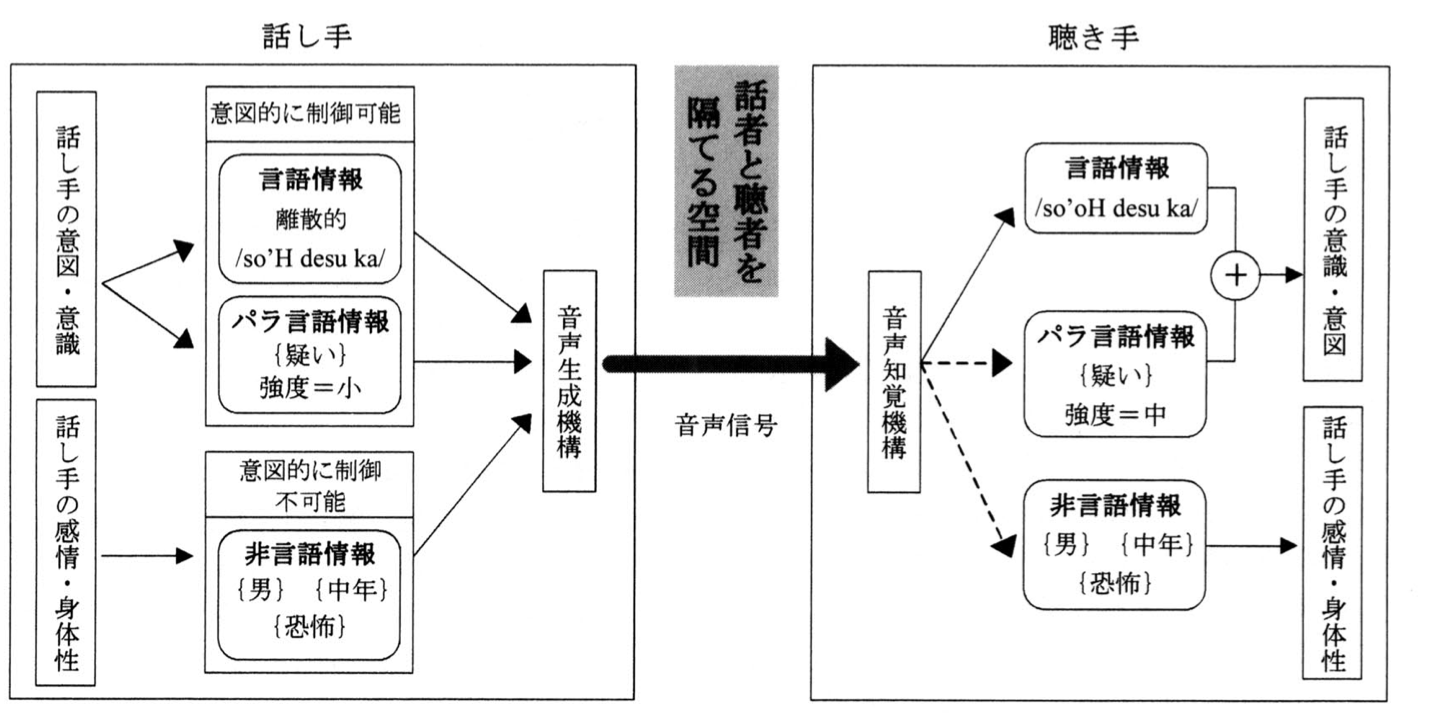
\includegraphics[width=12.0cm]{figures/maekawa_onsei.png}
 \caption[音声による情報伝達過程の模式図]{音声による情報伝達過程の模式図。 \cite{maekawa_onsei}より抜粋。話し手が聞き手へ言葉発した時の情報の伝達方法を模式的に表している。話し手発した情報の中でパラ言語情報と非言語情報が必ずしも正確には伝わらないことが示されている。 }
 \label{maekawa_onsei:fig}
\end{figure}

\newpage

\begin{figure}[hbtp]
 \centering
   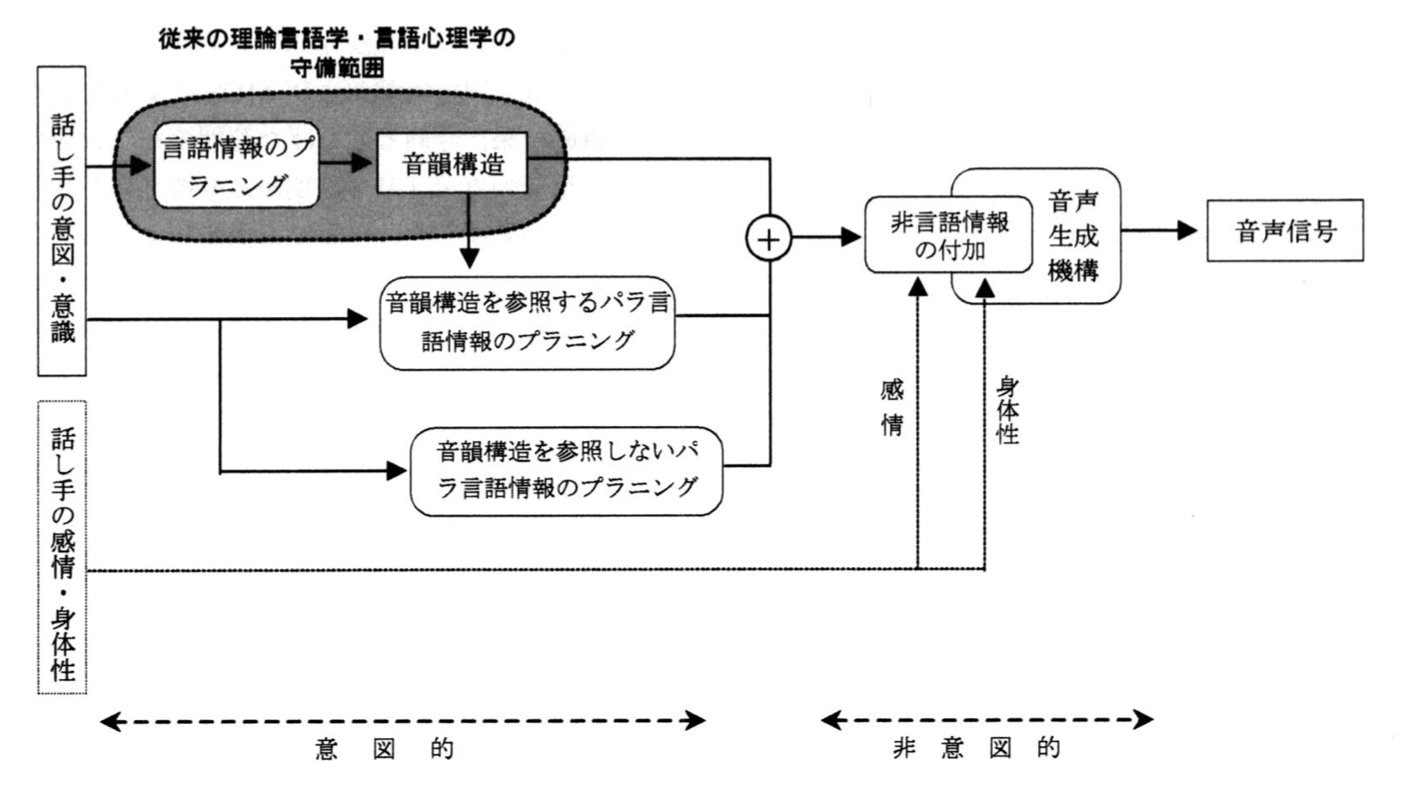
\includegraphics[width=12.0cm]{figures/maekawa_kitagawa.png}
 \caption[パラ言語情報を考慮した音声生成過程の模式図]{パラ言語情報を考慮した音声生成過程の模式図。 \cite{maekawa_kitagawa}より抜粋。 話し手が音声を発する時に、言語情報、パラ言語情報、非言語情報がどのように組み合わせて生成されているのかについて模式的に表されている。この画像から感情と身体性を含む非言語情報の付加は非意図的に生成されていることが示されている。 }
 \label{maekawa_kitgawa:fig}
\end{figure}


パラ言語情報を考慮した音声生成過程の模式図を図\ref{maekawa_kitgawa:fig}に示す。図\ref{maekawa_kitgawa:fig}によると、発話する際の音声に含まれる情報には意図的なものと非意図的なもが存在する。意図的なものには、パラ言語情報には音韻構造を参照するものと参照しないものに分けられる。このように音声のみに対してアプローチしている研究はなされているが、発話者同士の関係や発話者のスタイルに着目はされていない。

話した言葉が話し手の脳から聞き手の脳へ伝わる過程の模式図を図\ref{speech_chain:fig}に示す。図\ref{speech_chain:fig}では、話し手から発せられた音声と聴き手が音声を知覚するまでの過程がつながりを持っていることを示している。よって、話し手の意図と聴き手が知覚した内容には齟齬が生じることがある。ゆえに、パラ言語情報を認知すること自体やパラ言語情報の表現の仕方が曖昧なのである。

\begin{figure}[hbtp]
 \centering
   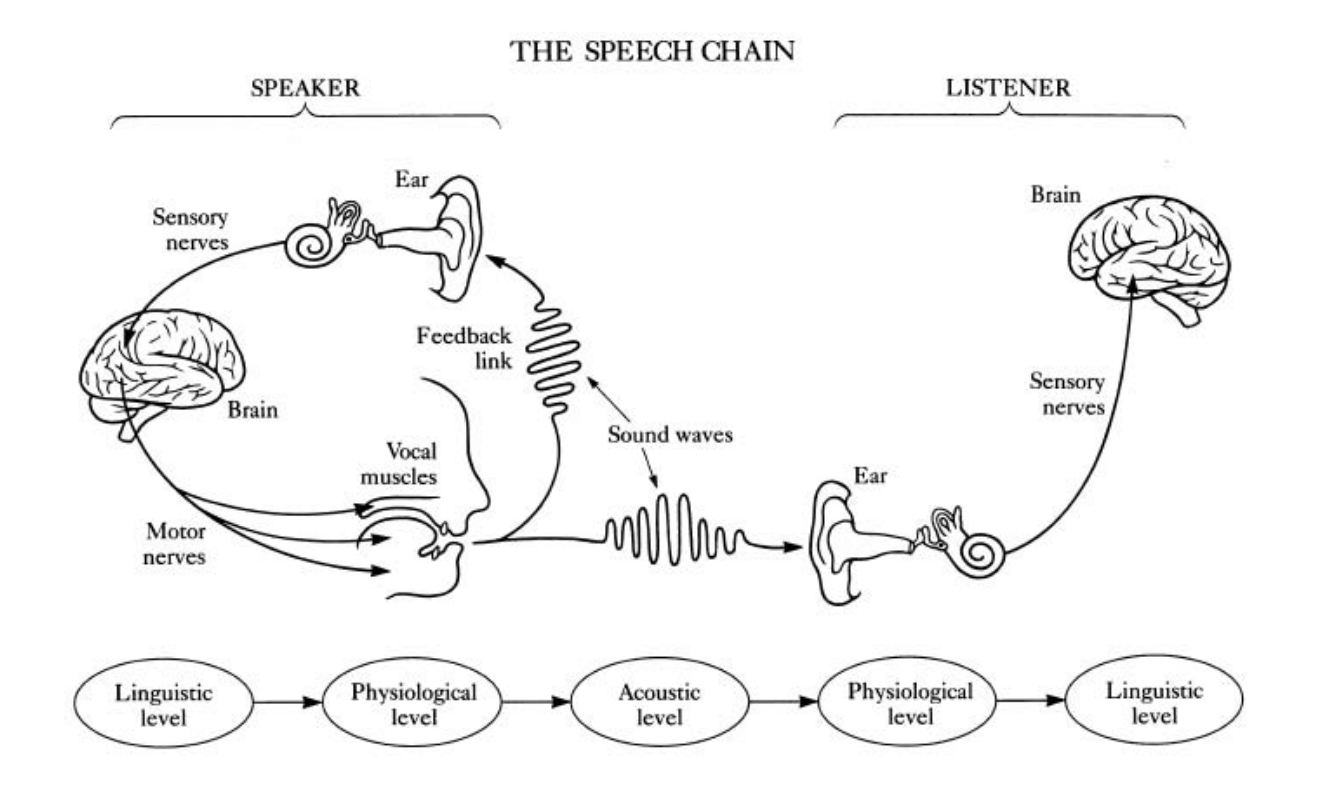
\includegraphics[width=12.0cm]{figures/speech_chain.png}
 \caption[The speech chain]{The speech chain。 \cite{speech_chain}より抜粋。話した言葉が話し手の脳から聞き手の脳へ伝わる過程が表されている。 }
 \label{speech_chain:fig}
\end{figure}





Wertschによると、自分の音声は他者の声から切り離されて存在するのではなく、発話が向けられる他者の声に基づいて作られるのである。また、音声は他者との関係において成り立つのであり、音声には状況依存性がある\cite{wertsch}。その状況とは、話し手と聴き手が物理的環境を共有することである\cite{maekawa_onsei}。
%このように発話は他者からの声に反応して発せられるものであるため、日常に現れる微細な音声の変化を分析するためには、対話音声を分析することが妥当である。

前川らによると、対話音声には、発話の重複・あいづち・語形の縮約・言いさし・言い直し・繰り返しなどの特微的現象が観察される。これらの多くは対話が複数の参加者による協働行為であることに起因している\cite{maekawa_inritsu}。さらに、石本によると、発話向け先との関係の違いによって日常対話の声の高さが変化することがわかっている。また、会話場面の同席者している参与者との関係によって韻律的多様性が生じていることがわかっている\cite{ishimoto}。発話向け先との関係の違いや同席しているを図\ref{ishimoto1:fig}に示す。図\ref{ishimoto1:fig}によると、家族に向けた発話は一般的に低い Fo で発声され、丁寧な発話ほど Fo が高くなることが読み取れる。つまり、対話相手によって発話スタイルが変わるため、パラ言語情報の表出の仕方が変わるのである。よって、パラ言語情報が発話者のみによって発せられるのではなく、発話相手によってパラ言語情報の表出の仕方が変わるため、音声のみに注目してはいけないと考えられる。音声のみに注目するのではなく、対話者の発話のスタイルや対話場面についても考慮すべきであると考えられる。


\begin{figure}[hbtp]
 \centering
   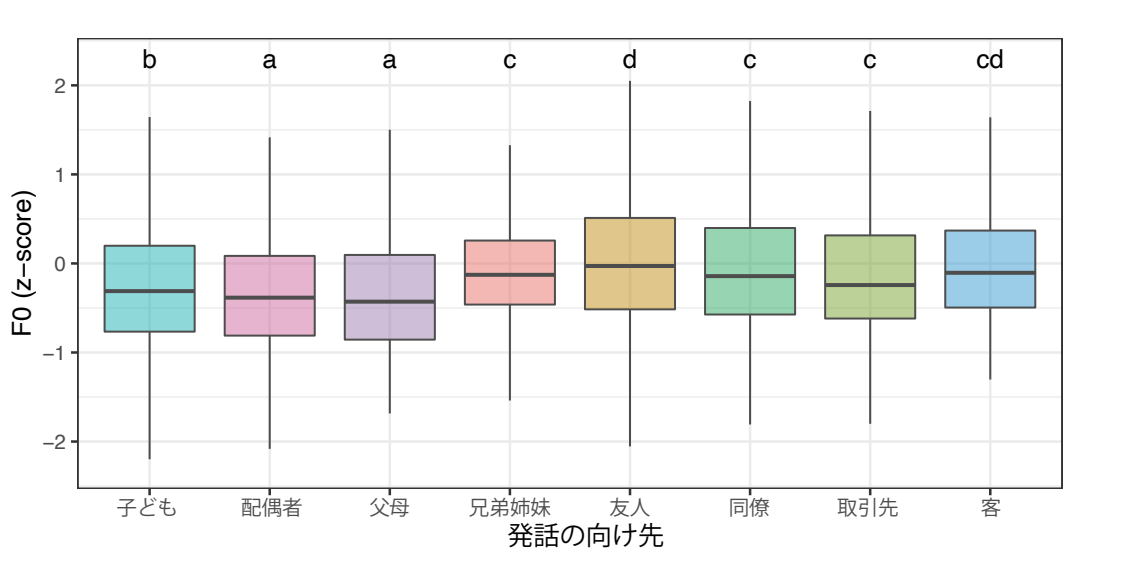
\includegraphics[width=12.0cm]{figures/ishimoto1.png}
 \caption[発話向け先ごとの発話の平均Foの分布]{発話向け先ごとの発話の平均Foの分布。 \cite{ishimoto}より抜粋。 }
 \label{ishimoto1:fig}
\end{figure}


%日本語日常会話コーパス

音響特徴量は感情ラベルに比べコーパスの特性の違いの影響を受け易いことがわかっている\cite{nagawaka_mori}。
よって、従来の対話音声研究では、パラ言語情報が収録したコーパスの特性の影響を受けやすいため、パラ言語情報を普遍的に明らかにするには至らなかった。
しかし、国立国語研究所では2016年より、日常生活の中で自然に生じる多様な場面・話者の会話 200 時間を対象とする『日本語日常会話コーパス』(CEJC)の構築が進んでいる\cite{koiso}。
多様な関係性における対話を収録した日常対話コーパスによって、コーパスの特性に限定されることなく対話音声を分析できるようになった。


%非流暢性について
自発発話には非流暢性が必ず伴う。よって、自発発話の分析には非流暢性の分析が必要であると考えられる。また、非流暢性は自発発話に現れるという特徴だけでなく、コミュニケーションにおいて様々な役割がある。先行研究では以下のように述べられている。聞き手に対して様々な影響を与える現象である。特に、フィラーは発話権を保持する役割を持っているおり、音韻の引き伸ばしは発話の中断の合図になっている\cite{den}。このように非流暢性はコミュニケーション方略として用いられていることはわかっている。しかし、非流暢性の全体像をカバーするような分析は行われていない。さらに、言語情報とパラ言語情報との間の交互作用について分析するべきであるということは、\cite{maekawa_kitagawa}でも述べられている。


\newpage


\subsection{目的}\label{section_mokuhyou}
本研究では、日常的かつ自然な対話音声と非流暢性の関係を明らかにすることを目指す。さらに、様々な関係性や発話のスタイルによってパラ言語情報の表出の仕方がどのように変化するのかを調べる。この目的を達成するために、次の三つのリサーチクエスチョンを設定した。

\begin{enumerate}
  \item 親密度の変化によって非流暢性はどのように変化するのか
  \item 非流暢性の出現頻度にはどのような傾向があるのか
  \item 対話において非流暢性が果たす役割の定量的な特徴はどのようなものか

\end{enumerate}

\subsection{波及効果}

パラ言語情報を構成する要素を明らかにすることで、パラ言語情報を分析する際の一つの指標として確立することができる。また、パラ言語情報の表出方法の仕組みを明らかにすることにもつながるであろう。さらに、スタイルの違いに応じたパラ言語情報の表出方法がどのようなものであるかを明らかにできる。その結果、場面に適した音声を使うことで、教育やトレーニングを行う際にも、どのような音声が指導に適切であるか知ることができる。それに加え、パラ言語情報についての知見を応用することで、音声合成、音声変換の多様性を実現できるであろう。


